\documentclass{article}
\usepackage[utf8]{inputenc}
\usepackage[T1]{fontenc}
\usepackage{graphicx}
\usepackage{hyperref}
\usepackage{geometry}
\geometry{margin=1in}

\title{ESCHEAT}
\date{Encyclopaedia Britannica (1771)}

\begin{document}
\maketitle

\section*{Historical source}
\textbf{Entry ID:} \texttt{entry-escheat-1473} \\
\textbf{Volume ID:} 149979622 \\
\textbf{Character Count:} 986

\subsection*{Extracted Text}
ESCHEAT, in law, signifies any lands or ten-
parts that cafinally fail to a Lord within his manor.
It is one of the confeugeures of tenure in divary
(See \_Fiona Sylpa, Amoran-Serous\_, and Texas).
If the determination of the course are diflutions
of the mutual bond between the loud and tenans, from
the extinction of the blood of the latter by other ana-
ural or crist means : if the deck without hers of his
blood, or if his blood the company and named by
comunition of coercion or fidory; whereby every hori-
britable quality was entirely blasted out and doubled,
fa fault, cakes the hand echated or fell back to the
lost of the cry that is, the teens was determined by
breach of the original condition, esperified or implied
in the fetal donation. In later once cats, there were
no here inhibiting of the blood of the fork tettatory
or puchader, to which hers alone the grant of the
feed extended: in the other, the tenant, by perpe-
trating an atrocious crime, showed that he was no



\section*{Source record}
\begin{itemize}
\item \textbf{Dataset:} \texttt{NationalLibraryOfScotland/encyclopaedia\_britannica\_illustrated}
\item \textbf{Dataset Revision:} \texttt{309f765b1ecc83e0a7f7762e44b4a927a7555443}
\item \textbf{Page ID:} \texttt{britannica:309f765b1ecc83e0a7f7762e44b4a927a7555443:train:1473} \\
  \textbf{Filename:} \texttt{page-1473-b3b602ef6a3d.jpg} \\
  \textbf{Row Index:} 1473 \\
  \textbf{SHA256:} \texttt{b3b602ef6a3d4961...}
\end{itemize}

\begin{figure}[h]
\centering
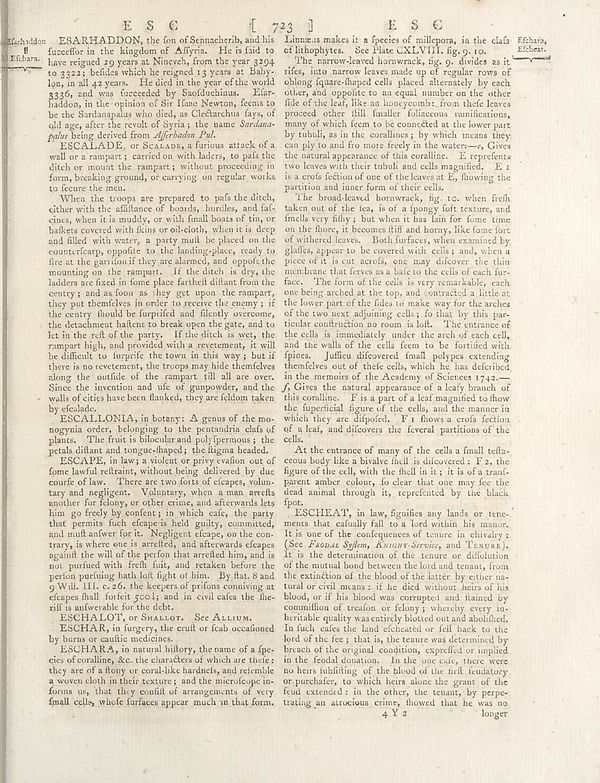
\includegraphics[width=0.85\textwidth]{../scans/page-1473-b3b602ef6a3d.jpg}
\caption*{Source scan: \texttt{page-1473-b3b602ef6a3d.jpg}}
\end{figure}

\end{document}
